\documentclass[a4paper]{article}
\usepackage[warn]{mathtext}
\usepackage[utf8]{inputenc}
\usepackage[T2A]{fontenc}
\usepackage[english,russian]{babel}
\usepackage{booktabs}
\usepackage{multicol}
\usepackage{fancyhdr}
\usepackage{graphicx}
\usepackage{microtype}
\usepackage{wrapfig}
\usepackage{amsmath}
\usepackage{floatflt}
\usepackage{geometry} \geometry{verbose,a4paper,tmargin=2cm,bmargin=2cm,lmargin=1.5cm,rmargin=1.5cm}
\usepackage{float}
\usepackage{amssymb}
\usepackage{caption}
\usepackage{epsfig}
\usepackage{newunicodechar}

\begin{document}

\graphicspath{ {pictures/} }
\begin{center}
    {\scshape\Large Лабораторная работа по твердотельной электронике} \par

    \

    {\huge\bfseries № 19. Исследование биполярных транзисторов.} \par 

    \

    {\large Яромир Водзяновский Б04-855а}
\end{center}

\

\

\section{Результаты}

\begin{figure}[H]
    \begin{center}
        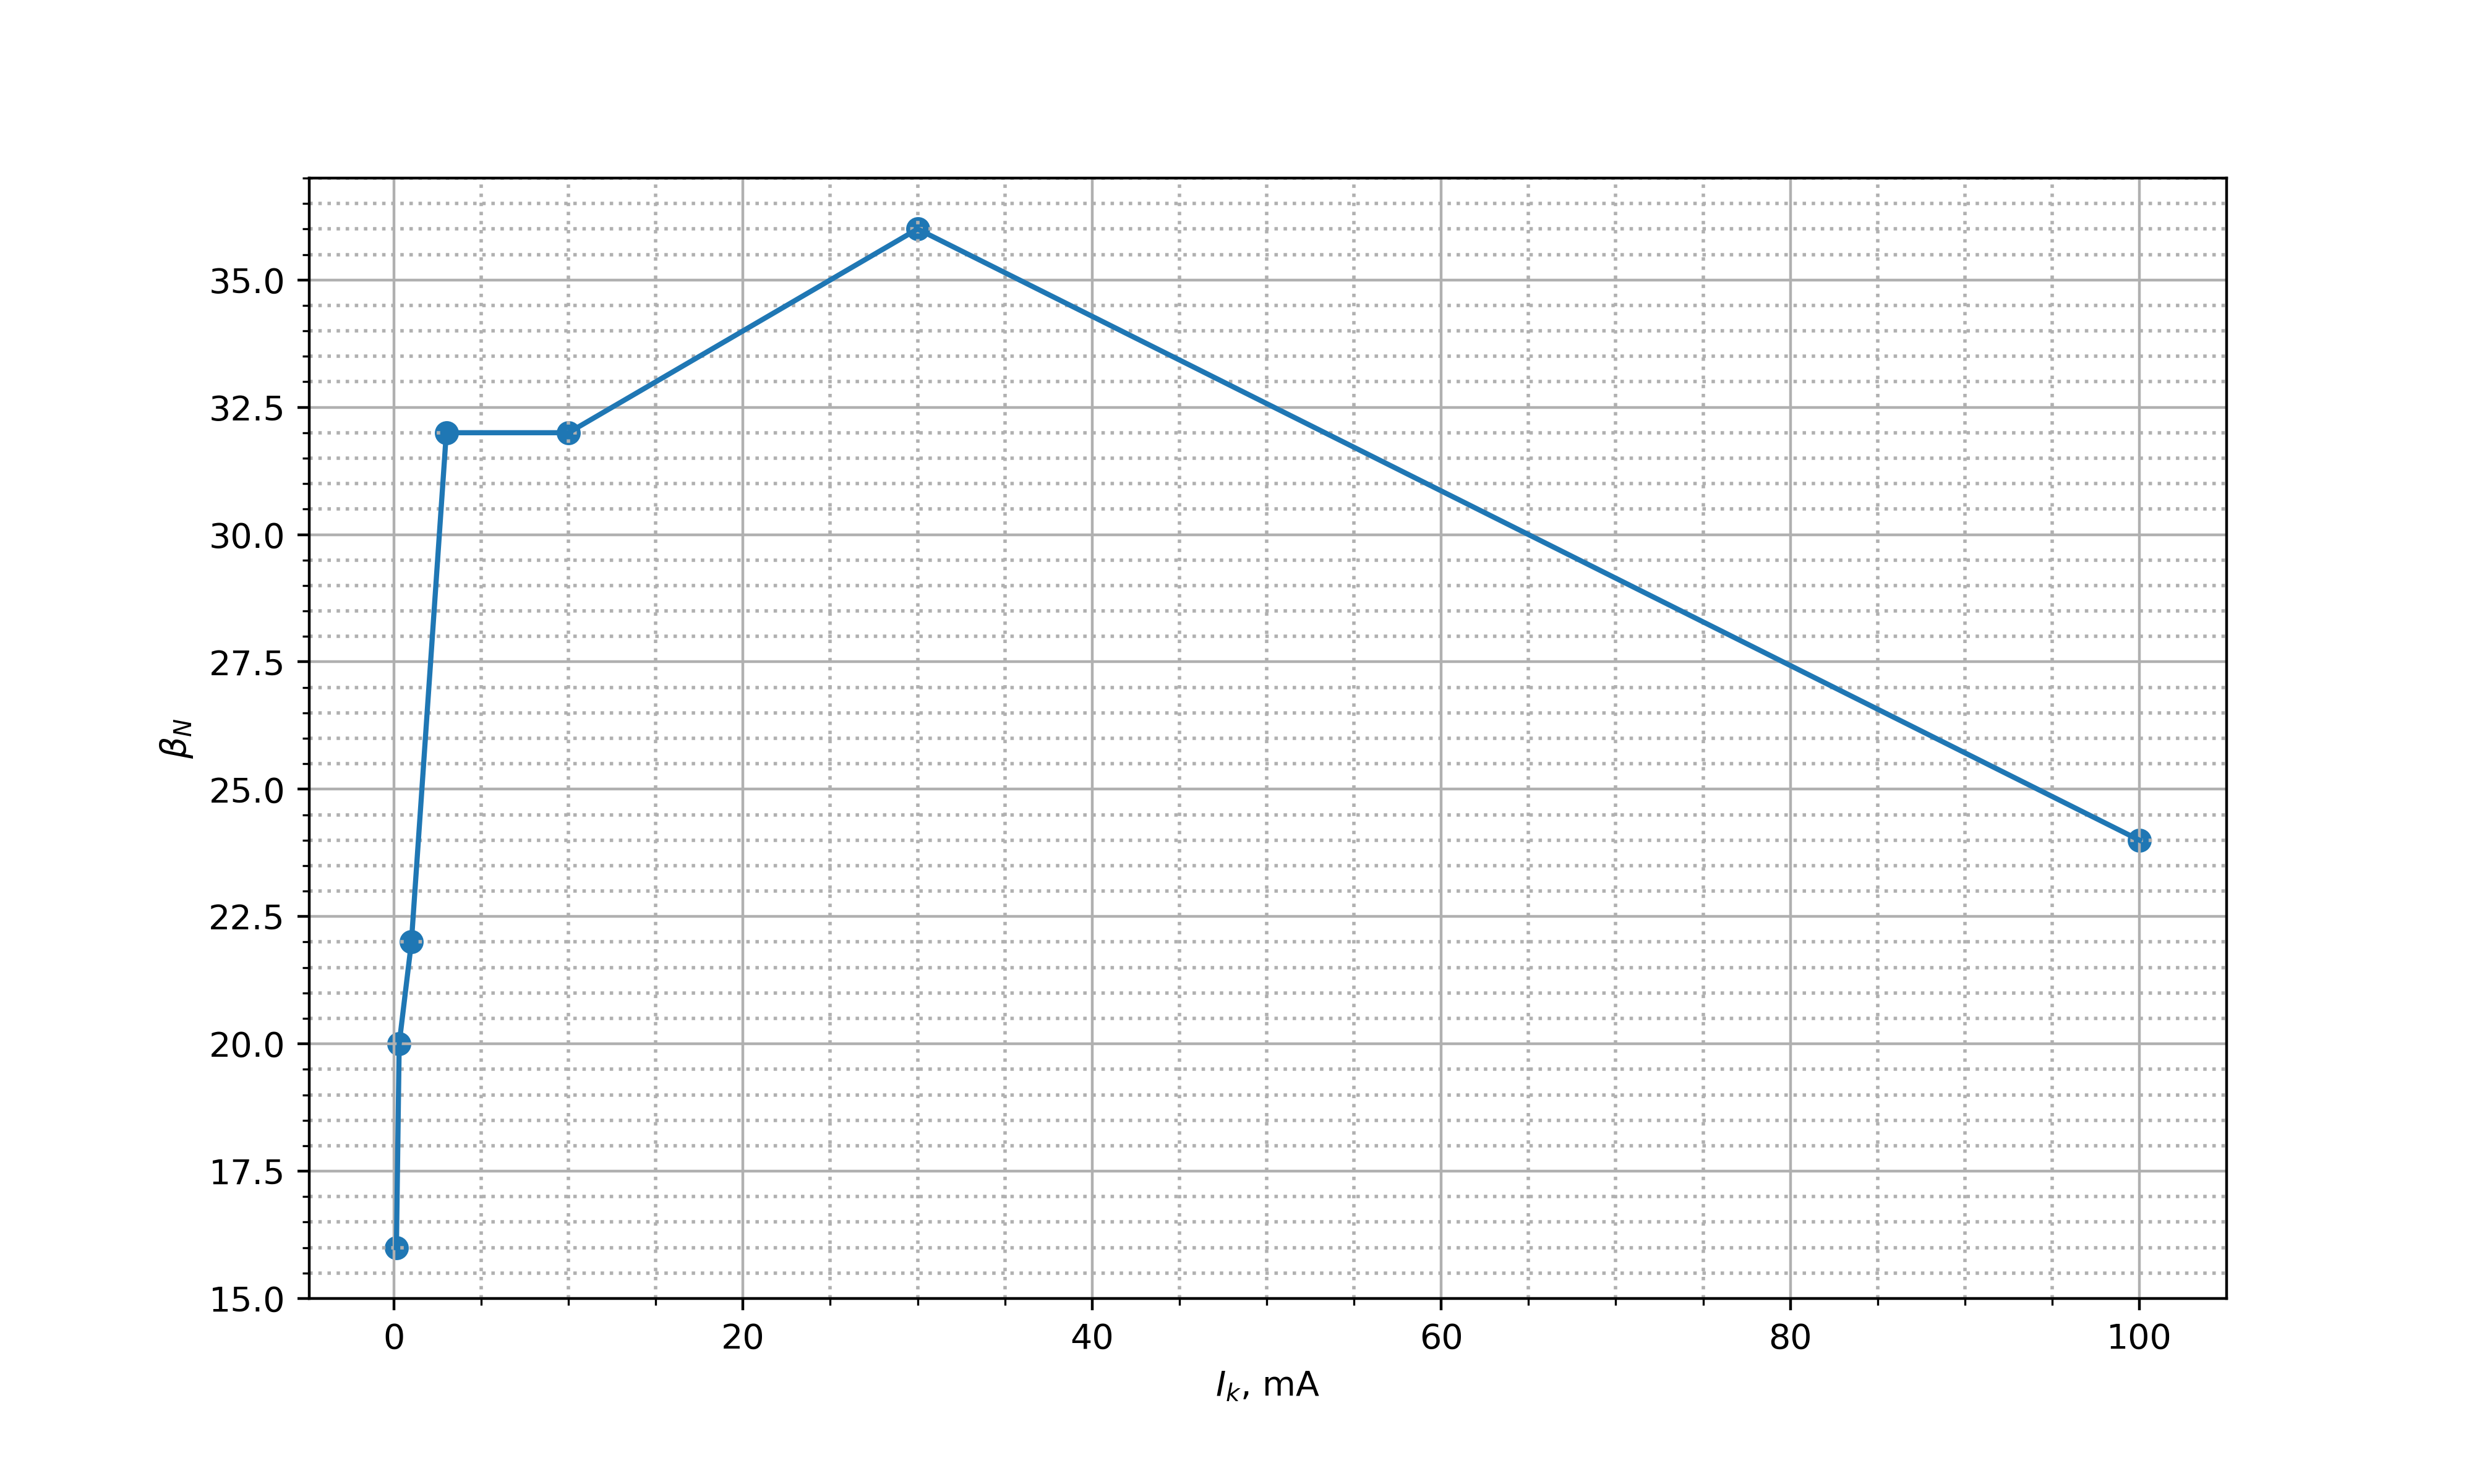
\includegraphics[scale = 0.8]{p1.png}
    \end{center}
    \caption{$\beta_N(I_k)$}
    \label{g1}
\end{figure}

\begin{figure}[H]
    \begin{center}
        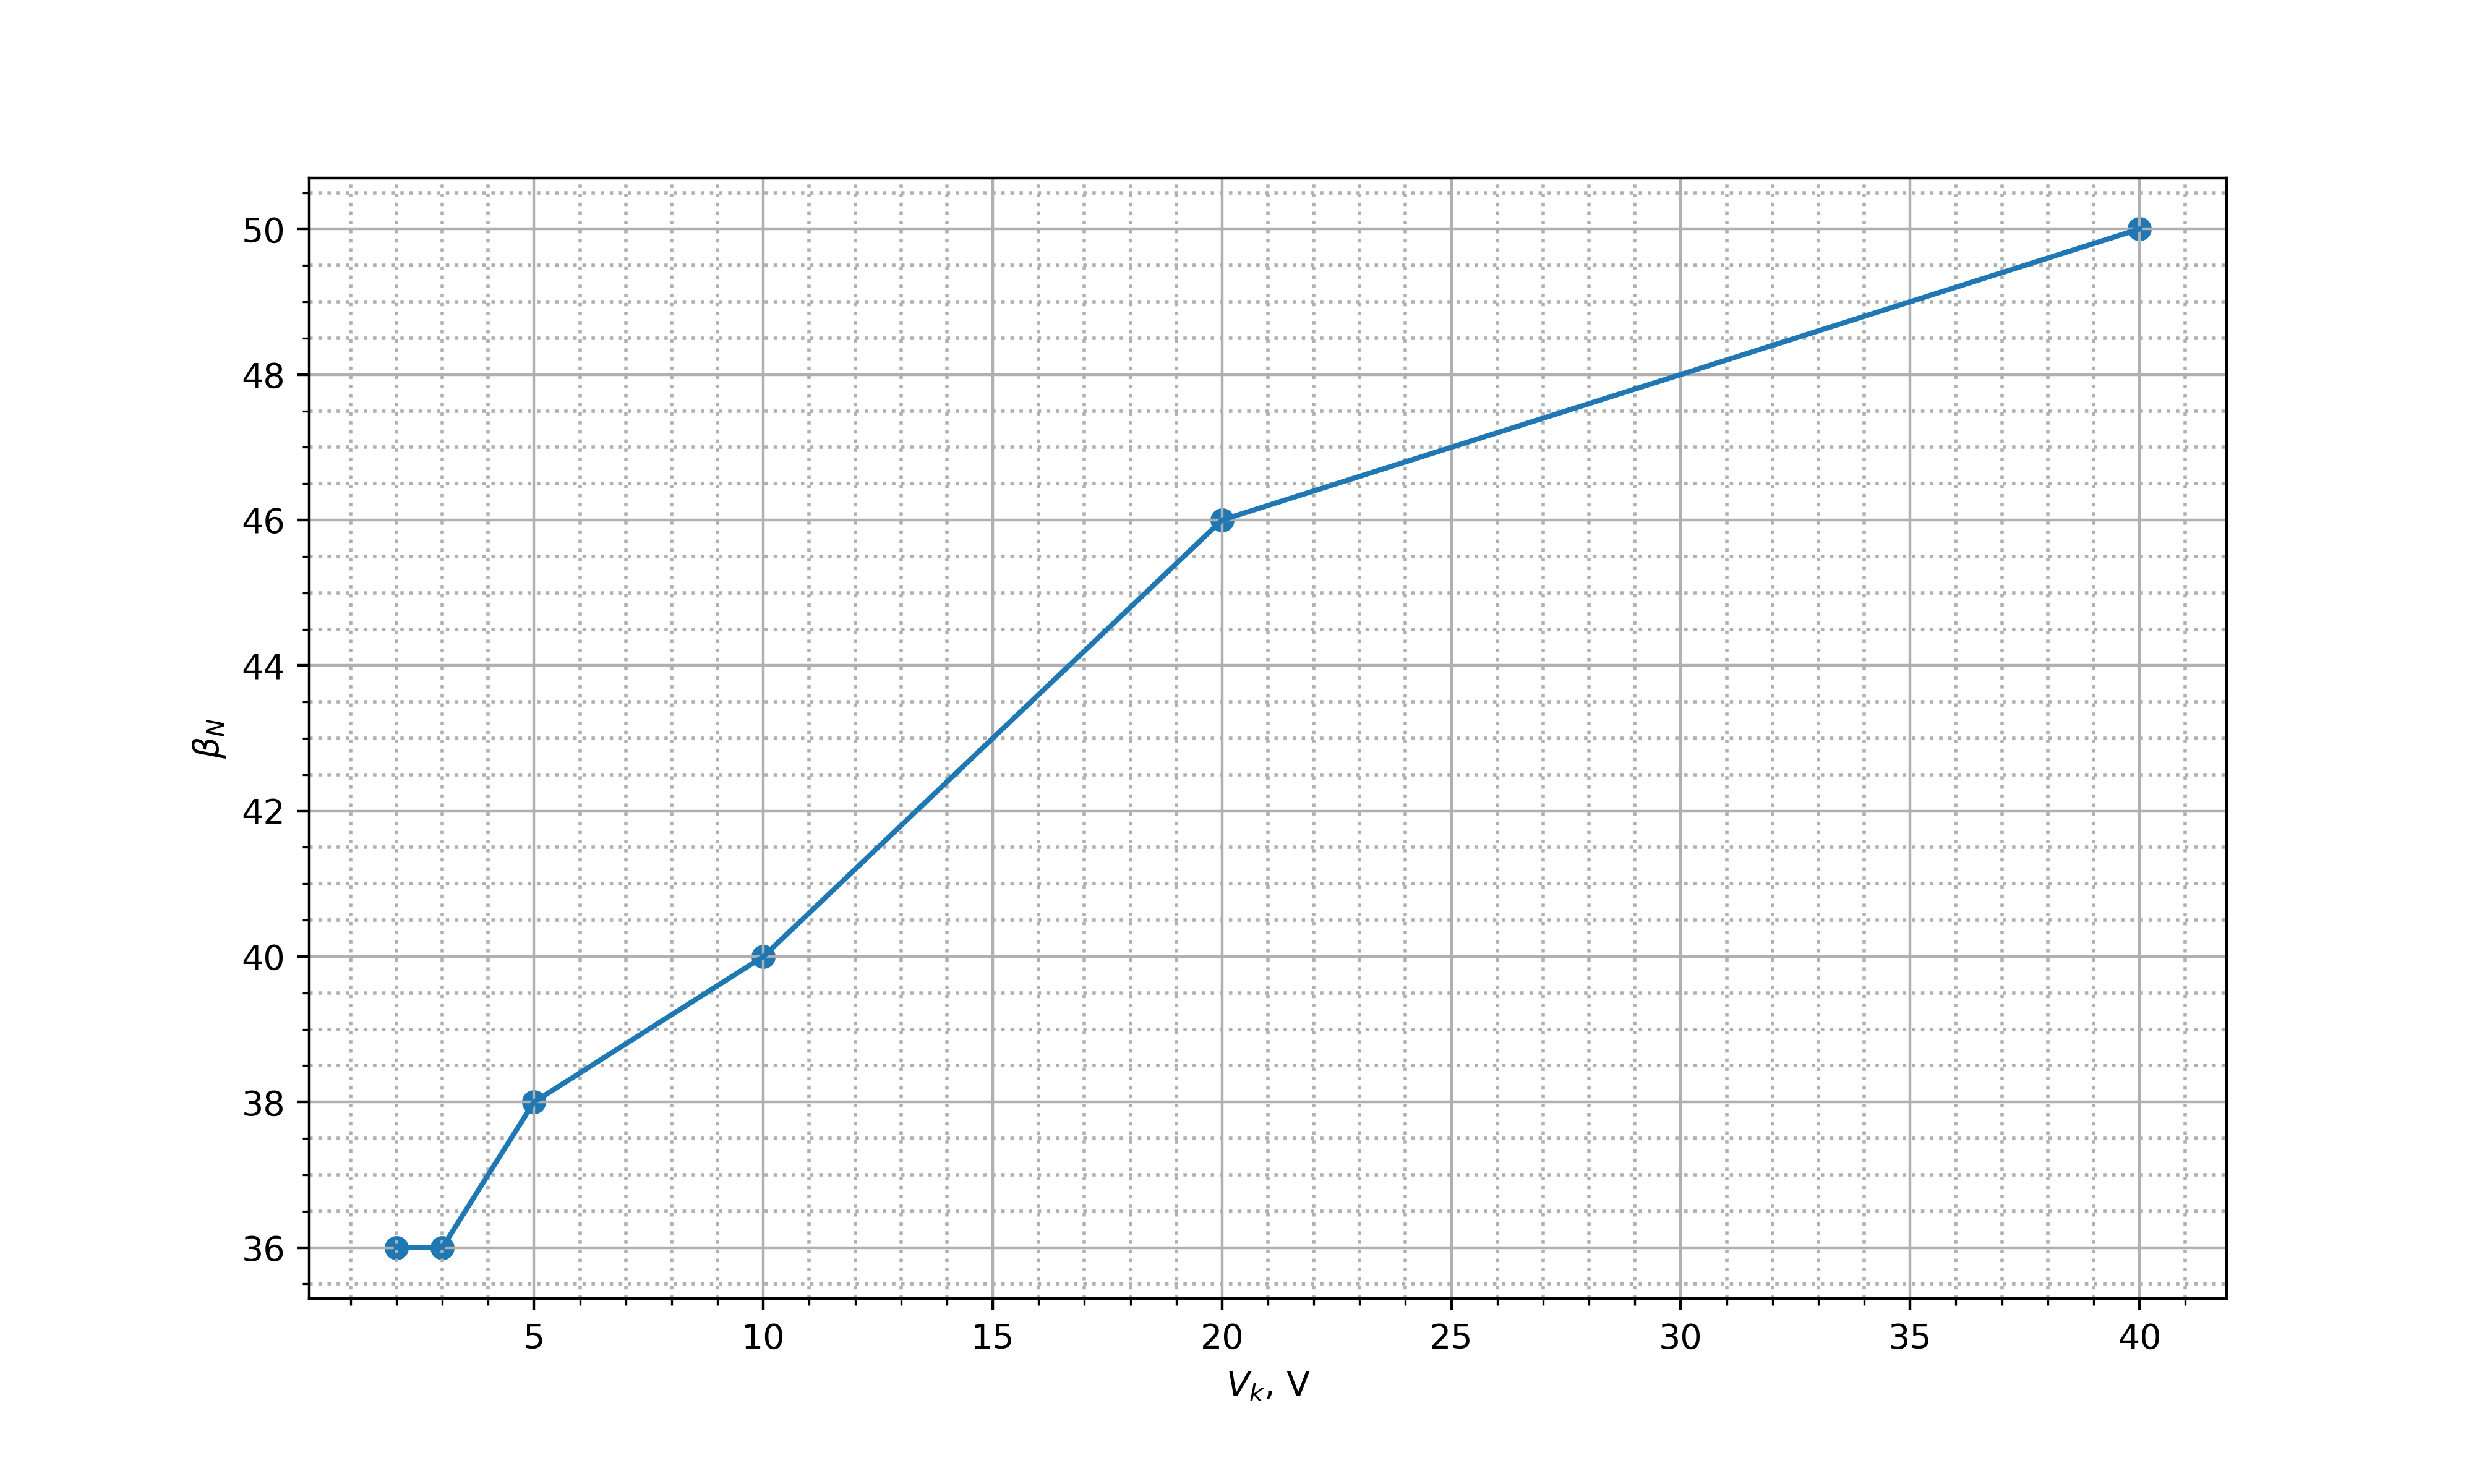
\includegraphics[scale = 0.8]{p2.png}
    \end{center}
    \caption{$\beta_N(V_k)$}
    \label{g2}
\end{figure}


\section{Эффект Эрли}

\textbf{Эффект Эрли} — влияние обратного напряжения на коллекторном переходе биполярного транзистора, работающего в активном линейном режиме на токи биполярного транзистора.  (эффект модуляции ширины базы при изменении коллекторного напряжения) \par 

\begin{figure}[H]
    \begin{center}
        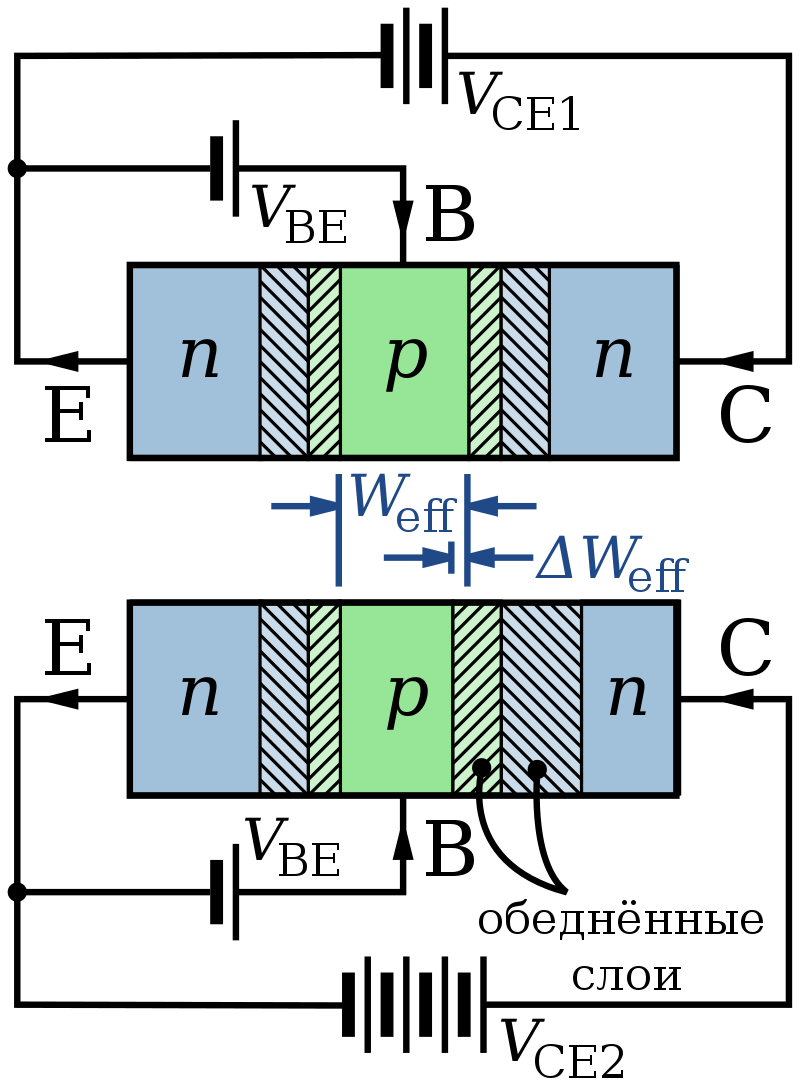
\includegraphics[scale = 0.2]{erli.png}
    \end{center}
    \caption{Эффект Эрли}
    \label{p1}
\end{figure}

Этот эффект проявляется в зависимости выходного дифференциального сопротивления каскада с общим эмиттером от напряжения 
$V_{CB}$ в активном режиме работы транзистора, также при увеличении 
$V_{CB}$ увеличивается коэффициент передачи тока базы.

Механизм возникновения этой зависимости следующий. При увеличении $V_{CE}$
коллекторный переход более сильно смещается в сторону запирания и при этом расширяется обеднённая зона коллекторного перехода за счёт уменьшения толщины базового слоя как показано на рисунке. Изменение напряжения на базе $V_{BE}$
относительно эмиттера (в прямосмещённом p-n переходе) при изменении управляющего тока незначительно изменяет ширину обеднённого слоя эмиттерного перехода и этим изменением можно пренебречь.

При сужении ширины базового слоя, вызванного изменением $V_{CB}$
снижается вероятность рекомбинации в суженном базовом слое и увеличивается градиент плотности объёмного заряда в базовом слое, что увеличивает коэффициент инжекции носителей заряда из эмиттера в базу. Но только первый из этих эффектов называют эффектом Эрли.
В результате снижается выходное дифференциальное сопротивление.ы


\end{document}